\documentclass{article}
\usepackage{pgfplots}
\usepackage{xcolor}
\pgfplotsset{compat=1.18}

\definecolor{barblue}{RGB}{54, 106, 146}
\definecolor{axisblue}{RGB}{54, 106, 146}
\definecolor{bggray}{RGB}{235,235,235}

\begin{document}

\begin{center}
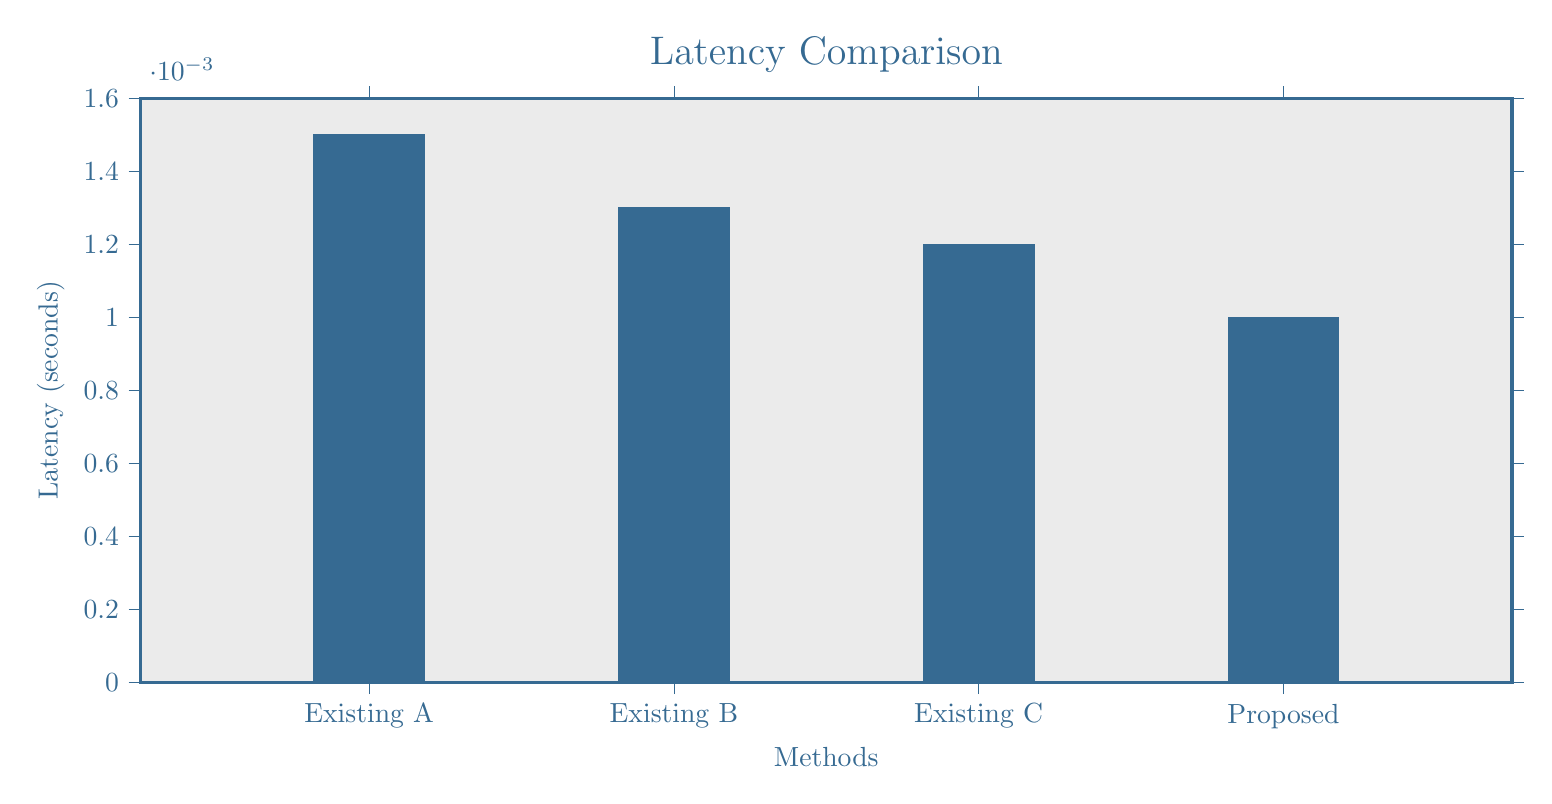
\begin{tikzpicture}
\begin{axis}[
    width=19cm,
    height=9cm,
    title={Latency Comparison},
    title style={font=\Large, color=axisblue},
    xlabel={Methods},
    ylabel={Latency (seconds)},
    xlabel style={color=axisblue},
    ylabel style={color=axisblue},
    tick label style={color=axisblue},
    xtick style={color=axisblue},
    ytick style={color=axisblue},
    axis line style={color=axisblue, line width=1.2pt},
    ymin=0,
    ymax=0.0016,
    symbolic x coords={Existing A, Existing B, Existing C, Proposed},
    xtick=data,
    bar width=40pt,
    enlarge x limits=0.25,
    ymajorgrids=false,
    grid=none,
    axis background/.style={fill=bggray},
    tick align=outside,
]

\addplot[
    ybar,
    fill=barblue,
    draw=barblue
] coordinates {
    (Existing A, 0.0015)
    (Existing B, 0.0013)
    (Existing C, 0.0012)
    (Proposed, 0.0010)
};

\end{axis}
\end{tikzpicture}
\end{center}

\end{document}
